\documentclass{standalone}
\usepackage{tikz}
\usetikzlibrary{arrows.meta, positioning, calc}

\begin{document}

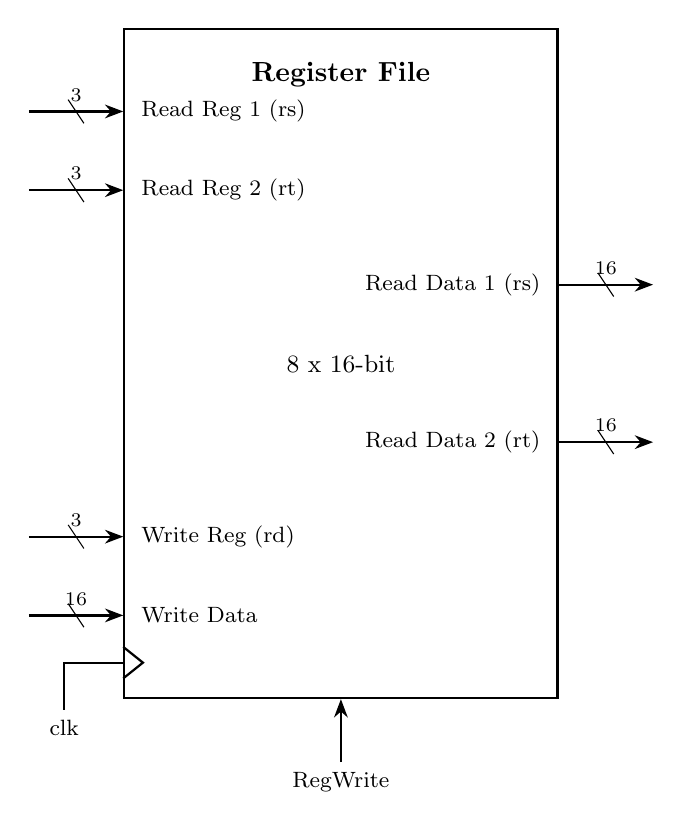
\begin{tikzpicture}[
    box/.style={rectangle, draw, minimum width=5.5cm, minimum height=8.5cm, thick, fill=white},
    port/.style={font=\footnotesize},
    label/.style={font=\scriptsize},
    arrow/.style={->, >=Stealth, thick}
]

    % Main Box - Height set to 8.5cm for clean spacing
    \node[box] (reg) at (0,0) {};
    
    % Header Title
    \node[font=\bfseries, yshift=-0.6cm] (title) at (reg.north) {Register File};
    
    % Center Capacity
    \node[font=\small] at (reg.center) {8 x 16-bit};

    % --- Left Side Inputs ---

    % Read Register 1
    \draw [arrow] ($(reg.west)+(-1.2, 3.2)$) -- ($(reg.west)+(0, 3.2)$)
        node[midway, above, label] {3}
        node[pos=1, anchor=west, port, xshift=0.1cm] {Read Reg 1 (rs)};
    \draw ($(reg.west)+(-0.7, 3.35)$) -- ($(reg.west)+(-0.5, 3.05)$); 

    % Read Register 2
    \draw [arrow] ($(reg.west)+(-1.2, 2.2)$) -- ($(reg.west)+(0, 2.2)$)
        node[midway, above, label] {3}
        node[pos=1, anchor=west, port, xshift=0.1cm] {Read Reg 2 (rt)};
    \draw ($(reg.west)+(-0.7, 2.35)$) -- ($(reg.west)+(-0.5, 2.05)$);

    % Write Register
    \draw [arrow] ($(reg.west)+(-1.2, -2.2)$) -- ($(reg.west)+(0, -2.2)$)
        node[midway, above, label] {3}
        node[pos=1, anchor=west, port, xshift=0.1cm] {Write Reg (rd)};
    \draw ($(reg.west)+(-0.7, -2.05)$) -- ($(reg.west)+(-0.5, -2.35)$);

    % Write Data
    \draw [arrow] ($(reg.west)+(-1.2, -3.2)$) -- ($(reg.west)+(0, -3.2)$)
        node[midway, above, label] {16}
        node[pos=1, anchor=west, port, xshift=0.1cm] {Write Data};
    \draw ($(reg.west)+(-0.7, -3.05)$) -- ($(reg.west)+(-0.5, -3.35)$);

    % --- Right Side Outputs (Evenly spaced from middle) ---

    % Read Data 1 (1.5cm above center)
    \draw [arrow] ($(reg.east)+(0, 1)$) -- ($(reg.east)+(1.2, 1)$)
        node[midway, above, label] {16}
        node[pos=0, anchor=east, port, xshift=-0.1cm] {Read Data 1 (rs)};
    \draw ($(reg.east)+(0.5, 1.15)$) -- ($(reg.east)+(0.7, 0.85)$);

    % Read Data 2 (1.5cm below center)
    \draw [arrow] ($(reg.east)+(0, -1)$) -- ($(reg.east)+(1.2, -1)$)
        node[midway, above, label] {16}
        node[pos=0, anchor=east, port, xshift=-0.1cm] {Read Data 2 (rt)};
    \draw ($(reg.east)+(0.5, -0.85)$) -- ($(reg.east)+(0.7, -1.15)$);

    % --- Bottom Control ---

    \draw [arrow] ($(reg.south)+(0, -0.8)$) -- (reg.south)
        node[pos=0, below, port] {RegWrite};

    % --- Clock Assembly ---
    \coordinate (clk_target) at ($(reg.west)+(0, -3.8)$);
    \draw [thick] ($(reg.west)+(-0.75, -4.4)$) node[below, port] {clk} 
          |- (clk_target);
    \draw [thick] ($(clk_target)+(0, 0.2)$) -- ++(0.25, -0.2) -- ++(-0.25, -0.2);

\end{tikzpicture}
\end{document}